 \documentclass[conference, 9pt, a4paper]{IEEEtran}
\usepackage[spanish, english]{babel}
\usepackage[utf8]{inputenc}
\usepackage{multicol}
\usepackage{amsmath}
\usepackage{amsfonts}
\usepackage{amssymb}
\usepackage{graphicx}
\usepackage{caption}
\usepackage{float}
\renewcommand\spanishtablename{Tabla}

\title{Calculo de Radio Enlace Terrestre 3G}
\author{
	\IEEEauthorblockN{	Amaya Matías }
	\IEEEauthorblockA{	Universidad Técnológica Nacional\\
						Legajo: 68284\\
						Email: matiasutn12@gmail.com\\
					}
	\and
	\IEEEauthorblockN{	Lamas Matías }
	\IEEEauthorblockA{	Universidad Técnológica Nacional\\
						Legajo: 65536 \\
						Email: @gmail.com\\
					}

	\and
	\IEEEauthorblockN{	Navarro Facundo }
	\IEEEauthorblockA{	Universidad Técnológica Nacional\\
						Legajo: 63809\\
						Email: facunava92@gmail.com\\	
					}
}

\begin{document}
\selectlanguage{spanish}
\maketitle  %ver el ttulo (y el autor)

\begin{otherlanguage}{english} 
\begin{abstract}
This article presents the calculation of radio link in the 3G band located in the Nueva Cordoba neighborhood of the city of Cordoba. To carry out the same, the COST 231-Walfisch-Ikegami propagation model was applied for a mobile channel located in an urban area.
\end{abstract}
\end{otherlanguage}

\begin{abstract}
Este articulo presenta el calculo de  radio enlace en la banda 3G ubicado en el Barrio Nueva Cordoba de la Ciudad de Cordoba. Para realizar el mismo   se aplico el modelo de propagacion COST 231-Walfisch-Ikegami para un canal movil ubicado en una zona urbana.

\end{abstract}

\section{INTRODUCCIÓN}
La propagación por radio  es esencial para las tecnologías emergentes con diseño apropiado, implementación y estrategias de gestión para cualquier red inalámbrica . Es muy específico del sitio y puede variar significativamente dependiendo del terreno, frecuencia de operación, velocidad del terminal móvil, fuentes de interfaz y otro factor dinámico.\\%% los dos porcentajes es para salitar linea
Los modelos de propagación  se pueden clasificar principalmente en dos extremos, es decir, completamente modelos empíricos y modelos deterministas.Los modelos empíricos se basan en datos medidos prácticamente.Hay algunos modelos que tienen las características de ambos tipos. Esos son conocidos como modelos semi empíricos
El modelo de Cost-231 Walfisch-Ikegami es categorizado como un modo semi empírico.\\
Estos modelos han sido ampliamente validado para redes móviles. La mayoría de estos modelos son basado en una interpretación sistemática de datos de medición obtenido en el área de servicio.\\

\section{MODELO \textit{Okumura-Hata}}
El modelo de Okumura es uno de los mas ampliamente utilizados para prediccion de señales en areas urbanas.\\
El principal resultado del trabajo de Okumura fue un conjunto de curvas que proporcionan el nivel de atenuación media relativa al espacio libre, en función de la frecuencia, la distancia entre transmisor y receptor, la altura de las antenas de la estación base y
la estación móvil, además de varios factores de corrección específicos para diferentes tipos de trayecto. Este modelo está considerado entre los más simples y mejores en términos de su precisión en el cálculo de las pérdidas en el trayecto y se ha convertido en uno de los más utilizados en la planificación de sistemas móviles de todo el mundo.

\begin{figure}
	\centering
	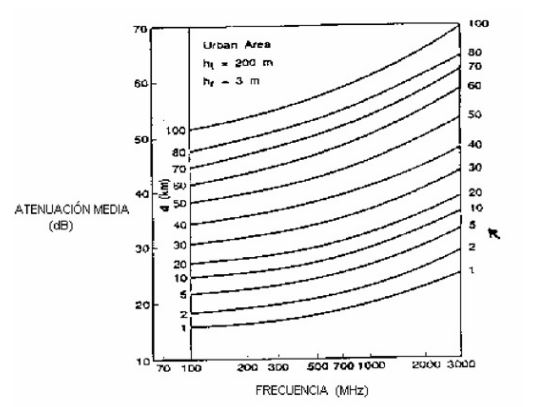
\includegraphics[width=\columnwidth]{image/okumura.JPG}
	\caption{Curvas de atenuación}
\end{figure}
Con el objetivo de hacer que este método fuera más fácil de aplicar, Hata estableció una serie de relaciones numéricas que describen el método gráfico propuesto por Okumura. Dichas expresiones de carácter empírico, son conocidas bajo el nombre de modelo de Okumura-Hata, también llamado modelo de Hata. Aunque éste no incluye ninguno de los factores de corrección por tipo de trayecto, los cuales sí están en el modelo de Okumura, las ecuaciones propuestas por Hata tienen un importante valor práctico. Este modelo es aplicable bajo las siguientes condiciones.



%hacer una tabla 
\begin{table}
\centering
\begin{tabular}{|c|c|}\hline  % hline indica la fila   c c son las columnas centradas  
	PARAMETROS							& RANGO	\\ \hline   %primero hago un salto de linea y despues indico la fila 
	Frecuencia Fc						& 100-1500 [MHz] \\ \hline 
	Altura de la estacion base			& 3 - 200  [m] \\ \hline 
	Altura de la antena movil			& 1 - 10   [m] \\ \hline
	Distancia de la antena al receptor  & 1 - 20   [Km] \\ \hline
\end{tabular}
\caption{Condiciones modelo OKUMURA-HATA}
\end{table}





\section{MODELO COST 231\textit{Walfisch-Ikegami}}
Este modelo, propuesto en el proyecto europeo COST 231, es resultado de la integración de los modelos de Ikegami-Ioshida y de Walfisch-Bertoni . En él se incorpora la influencia de edificaciones y calles en las que se encuentra el dispositivo receptor, para una predicción más precisa de las pérdidas de propagación en entornos urbanos.Este modelo es aplicable bajo las siguientes condiciones.\\
\begin{table}
	\centering
	\begin{tabular}{|c|c|}\hline
		PARAMETROS							& RANGO \\ \hline
		Frecuencia Fc						&  800 - 2000 [MHz] \\ \hline
		Altura de la estacion base			& 4 - 50   [m] \\ \hline 
		Altura de la antena movil			& 1 - 3    [m] \\ \hline
		Distancia de la antena al receptor	& 0,02 - 5 [Km] \\ \hline
	\end{tabular}
	\caption{Condiciones modelo COST 231 \textit{Walfisch-Ikegami}}
\end{table}


\section{DESARROLLO}

Se utilizara un canal de comunicaciones de la red 3G de telefonia de la compañia ``Claro" para llevar a cabo los calculos del enlace donde tenemos una antena transmisora-repetidora ubicada en la proximidad de la vivienda de uno de los integrantes del grupo.\\
Debido a que la distancia que entre la antena transmisora
y el receptor con la que se desea llevar a cabo este practico es de aproximadamente 177 m, es decir menor a 1 km, el modelo Okumura-Hata queda descartado, prosiguiendose a utilizar el modelo  COST 231 Walfisch-Ikegami.\\



\begin{figure}
	\centering
	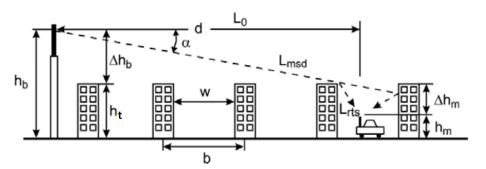
\includegraphics[width=\columnwidth]{image/GRAFICAAA.PNG}
	\caption{ COSTE 231 Modelo Walfish-Ikegamin}
\end{figure}




La ecuaciones que representa este modelo son las siguientes.\\
\begin{center}
 L(db) =\ Lo\ +\ Lrts\ +\ Lmsd 
\end{center}
Donde:\\
Lo: son las perdidas en espacio libre\\
Lrts: son las pérdidas por disfracción en los techo de las edificaciones. \\
Lmsd: son las pérdidas por disperción.\\
\begin{center}
 Lo= 46,2+26.log(d)+20.log(fc)
\end{center}
Donde:\\
d: es la distancia desde la antena y el receptor.\\
fc: es la frecuencia de la portadora . \\

\begin{center}
Lrts=-16,9-10.log(W)+10.log(fc)+20.log($\Delta $hm)+Lori
\end{center}
Donde:\\
W: es el ancho de la calle.\\
Lori: pérdida según el ángulo que llega la señal al móvil.
En nuestro caso el ángulo de incidencia es de  30°, utilizamos la siguiente expresion .\\
\begin{center}
Lori= -10 + 0,354.$\phi$[grados]
\end{center}
\begin{center}
Lmsd = Lbsk +ka+ Kd.log(d)+Kf.log (fc)-9.log(b)
\end{center}
Donde:\\
Lbsk : es un término que depende de la altura de la estación
base\\
Ka: representa el incremento de la pérdida en el trayecto
para el caso de estaciones bases ubicadas por debajo de la
altura media de los edificios.\\
Kd: dependencia de Lmsd con la distancia .\\
Kf : dependencia de Lmsd con la frecuencia . \\ 
b:  distancia promedio entre edificios. \\


\section{ANTENA Y RECEPTOR}
La antena seleccionada para la realizacion de los respectivos
calculos se encuentra ubicada en el barrio nueva cordoba y cuyas caracterısticas y coordenadas son: 



\begin{figure}
	\centering
	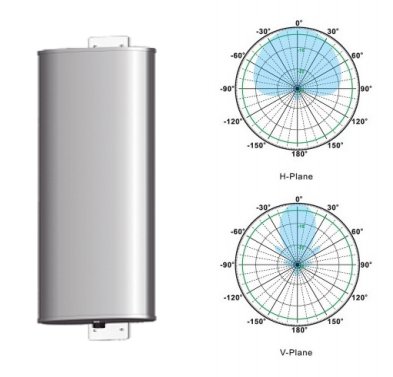
\includegraphics[width=\columnwidth]{image/ANTENA.PNG}
	\caption{ Antena  Marca TXPRO modelo TX9181290NFn}
\end{figure}


\begin{table}
\centering
\begin{tabular}{|c|c|}\hline  
	Rango de Frecuencia					    & 806 - 960 / 1710 - 1990 [MHz] \\ \hline 
	Ganancia								& 12 dBi / 12 dBi \\ \hline 
	Apertura(Horizontal / Vertical)			& 83° / 30° / 90° / 30° \\ \hline
	Polarización 							& Vertical \\ \hline
	Dimensiones								& 112.7 x 26.9 x 12.9  [cm] \\ \hline
\end{tabular}
\caption{Caracteristicas de la Antena}
\end{table}





Mediante la utilizacion de la aplicacion Google Maps se determinara la distancia real entre la antena y el receptor, siendo la misma 176,94 m.
\begin{center}
 Coordenadas del Receptor 
 \end{center} 
Latitud : 31°25'46.68"S\\
Longitud : 64°11'11.66"O \\
\begin{center}
 Coordenadas de la Antena
 \end{center} 
Latitud :31°25'50.53"S\\
Longitud :  64°11'6.67"O \\





\begin{figure}
	\centering
	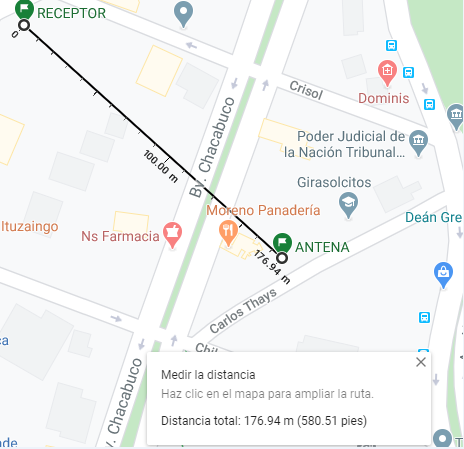
\includegraphics[width=\columnwidth]{image/Captura.PNG}
	\caption{Ubicacion Geografica}
\end{figure}


En cuanto a la frecuencia, para 3G es necesario que el
dispositivo receptor (o nuestro telefono, en este caso) soporte las dos bandas de frecuencia (UMTS 850 y UMTS 1900), debido a que esto es lo que se encuentra rigiendo vigente tanto en la ciudad de Cordoba como en el resto de Argentina y,de esta forma, nos aseguramos conectividad con cualquier antena del pais.


\begin{table}
\centering
\begin{tabular}{|c|c|}\hline  
	fc=850 MHz					  & Frecuencia Portadora \\ \hline 
	hb=38 m						   & Altura estacion base \\ \hline 
	hm = 1,50 m			          & Altura antena movil \\ \hline
	d= 0,17694 Km 				& Distancia movil-base \\ \hline
	Ptx = 40 dBm				& Potencia Transmisor \\ \hline
	Gtx=12 dBi					 & Ganancia Antena Tx \\ \hline 
	Grx=2 dBi					& Ganancia Antena Rx \\ \hline 
	Lctx = 1 dBi				& Perdida conectores Tx \\ \hline
	Lcrzx= 1 dBi 				& Perdida conectores Rx \\ \hline

\end{tabular}
\caption{asdasd}
\end{table}







\section{RESOLUCION}
Calculo de Lo :\\
Lo= 46,2+26.log(d)+20.log(fc)= 85,235\\\\
Calculo de Lrts donde tenemos :\\
W=4,3 m\\
fc = 850 MHz\\
$\Delta $hm = 23,5 m\\
Lrts=-16,9-10.log(W)+10.log(fc)+20.log($\Delta$hm)+Lori=34,10dB\\
\\
Calculo de Lmsd:\\
Lmsd = Lbsk +ka+ Kd.log(d)+Kf.log (fc)-9.log(b)\\
Para nuestro caso:\\
b:  distancia promedio entre edificios.\\
Lbsk= 0 dado que la altura del techo es mayor a la de la antena .\\
Ka= 54 - 0,8.($\Delta$Hbase).($\dfrac{d}{0,5}$), dado que la altura del techo es  mayor a la de la antena y d$<$0,5 Km.\\
Kd=$ 18\ -\ 0,\ 8.\left( \ \ \frac{\Delta Hbase}{Htecho} \ \ \ \right)\ $,  dado que la altura del techo es mayor a la de la antena.\\
Kf=$\ -4\ +\ 1,\ 5\ .\left( \ \ \frac{Fc}{925} \ -1\ \ \right)$ dado que se trata de un centro metropolitano.\\

Lmsd=Lbsk+ka+Kd.log(d)+Kf.log(fc)-9.log(b)=17,893dB\\

Luego de realizar los reemplazos y las operaciones matemáticas correspondientes, obtenemos la atenuación en el espacio libre, la cual es igual a:\\
\begin{center}

L(db) =\ Lo\ +\ Lrts\ +\ Lmsd= 137,229 dB
\end{center}
El nivel de señal recibido sera igual a:\\
\\
Nivel=Ptx-Lctx+Gtx-L+Grx-Lcrx+Grx=-83,22 dBm\\
\\

Mediante la utilizacion de la aplicacion Network Cell Info Lite se puede corroborar el resultado obtenido.


\begin{figure}
	\centering
	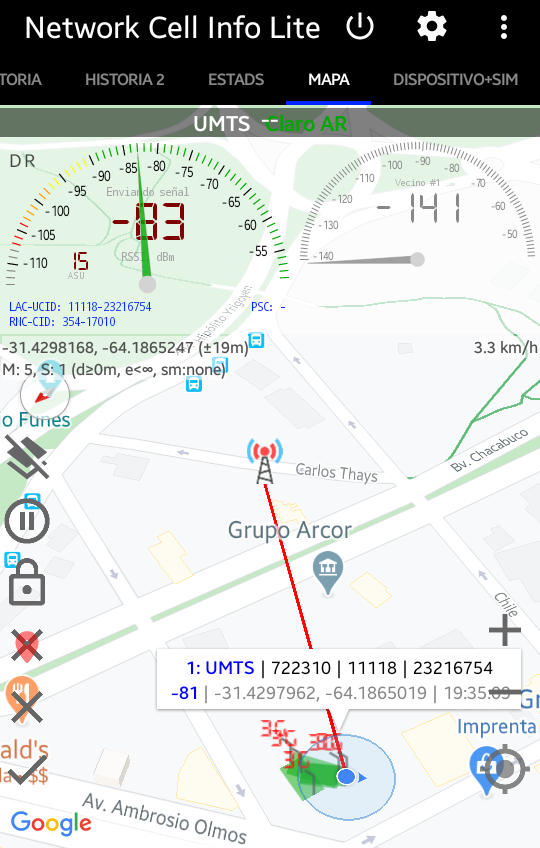
\includegraphics[width=\columnwidth]{image/Screenshot_2020-06-26-19-35-34-1.png}
	\caption{ Enlace}
\end{figure}



\section{CONCLUSION}
En el presente páctico se realizo el cálculo de el nivel de recepción de señal.
Hay que tener en cuenta que al momento de llevarse a cabo dicho metodo se estimo una antena base con una potencia de transmision de 40dB.
Pueden observarse que el resultado  arrojado concuerda con el valor  de nivel de recepción obtenidos en el movil.En el 
modelo COST 231 puede observarse una fuerte dependencia del nivel de atenuación de trayecto con el ancho de las calles donde se propagara la señal.
Es trabajo se  aprendió  sobre la existencia y el uso de distintas aplicaciones  para conocer la ubicación de la antena transmisora y  los niveles de señal recibidos. 
%Vamos a necesitar unas series de herramientas que detallaremos a continuacion para poder realizar el culculo.\\

%\textbf{1.} Un telefono movil que opere en la banda 3G ,es necesario que el dispositivo )soporte las dos bandas de frecuencia (UMT 850 y UMTS 1900), que son que se encuentran vigente en la ciudad de Cordoba\\

%\textbf{2.} Aplicacion movil que permite corroborar los niveles de señal recibido , como identificar la celda que proporciona el servicio, en nuestro caso vamos a utilizar la app Network Cell info Lite\\












%saco la ecuacion de https://www.mathcha.io/editor
%\begin{equation}
%\frac{asd\ +\ asd\ }{asdasd}   
%\end{equation}


%– This article presents the study of the operating 
%	\[c=\frac{qw}{rtrt} \dfrac{asd }{ere} \]  %tiene q terminae en \] 	
%	\begin{equation}   %entre a ecuacion enumerada
%	2^{45} 
%	\end{equation}
	
	%imagen incerar



%\begin{center}
%Fig5 : matiasdasdasd
%\end{center}
%asdajfójo´fjasfasf


 
\begin{thebibliography}{99} %enumerar automatico numero de bibiografias  %referencias el titulo auto 

\bibitem{} {Electromagnetic Wave Interactions
Por Ard shir Guran, Raj Mittra, Philip J. Moser}

\bibitem{} {Raj Jain, «Channel Models: A Tutorial», 2007}

\bibitem{} {Quintana, Bordón Lopez, Montejo Sanchez, «Estudio comparativo de los
modelos de propagación de canal inalámbrico», Universidad Central de
Las Villas (UCLV), Cuba}

\end{thebibliography}

\end{document}







